\documentclass{llncs}

%% Verwende A4-Format statt Letter
\usepackage{a4}
%% Deutsche Silbentrennung und Sprache (neue Rechtschreibung)
\usepackage[ngerman]{babel}
%% Verwende Schriftart mit "echten" Umlauten statt Akzenten
\usepackage[T1]{fontenc}
%% Verwende Umlaute direkt
\usepackage[utf8x]{inputenc}
%% Hyperlinks für interne Referenzen
\usepackage{hyperref}
%% Grafiken einbinden
\usepackage{graphicx}
%% Paket für Unterabbildungen pro Abbildung
%\usepackage{subfig}

% Titel der Arbeit
\title{Peer-To-Peer in Botnets}

% Angaben zum Author
\author{Moritz Marc Beller,\\Ben Nachname}
\institute{%
   Fakultät für Informatik, \\
   Technische Universität München \\
%    Munich, Germany\\
   \email{\{beller,bennachname\}@in.tum.de}
}

\pagestyle{plain}

%------------------------------------------------------------------------------
\begin{document}

\maketitle

%------------------------------------------------------------------------------
\begin{abstract}
Diese Arbeit behandelt ein interessantes Thema.
\end{abstract}

%------------------------------------------------------------------------------
\section{Einleitung}



\section{Definitions}
A computer able of executing remotely-triggered commands is called a
{\it bot} or {\it zombie.} A {\it botnet} is a group of bots forming a
common network structure.\cite{schoof2007detecting} In most recent
papers on the subject (\cite{wang2009systematic},
\cite{abu2006multifaceted}), the term botnet is defined as purely
negative, i.e. a network performing destructive aims such as
denial-of-service attacks attacks, sending spam or hosting a phishing
website\cite{steggink2007detection}. Other common aims include
providing the aggregated CPU resources of the botnet, stealing user's
credentials \cite{borgaonkar2010analysis} or doing click fraud on
affiliate networks\cite{clickFraud}. We'd like to propas a bias-free
definition of botnet as per our understanding technology is generally
ethics-free. Additionally, there are many examples where botnets are
used in a non-destructive way (e.g. \cite{seti}), or even to destroy
existing ``evil-minded'' botnets.

A {\it botmaster} is referred to as the controller of the botnet. This
doesn't necessarily have to be the founder of the botnet (cf. \ref{ClassificP2P}).

The expression {\it bot candidates} specifies the set of computers
which are target to becoming a bot themselves.

{\it Peer-to-Peer}, being a technology buzz word of the internet in
the late 1990s with file sharing services like Napster\cite{napster},
has attracted less attention in recent years. {\it P2P } defines an
unstructured information network amongst equals --- so-called
peers. Two or more peers can spontaneously exchange information
without a central instance. According to \cite{schoder2005core} ``P2P
networks promise improved scalability, lower cost of ownership,
self-organized and decentralized coordination of previously underused
or limited resources, greater fault toler- ance, and better support
for building ad hoc networks.''  These properties coupled with the
fact that files circumfloating in P2P networks are prone to malware,
trojans and viruses make P2P networks a most-attractive base for
building botnets.  Well-known P2P networks include the
Napster\cite{napster}, Gnutella, Overnet and Torrent network.  A {\it
  P2P bot} then is a bot that uses a P2P protocol as a means of
communication with other bots.

The so-called {\it C\&C}, command and controll structure, specifies
the way and protocols in which the botmaster and the bots communicate
with each other. It is the central property of any botnet. Common
protocols for C\&C include IRC, HTTP, FTP and P2P.\cite{borgaonkar2010analysis}

{\it IRC} --- internet relay chat --- is a ``teleconferencing
system''\cite{irc}, typically used for text chatting in channels
joined by a large number of participants. While its protocol is
relatively easy to implement, it provides a lot of features. It has
thus become the de-facto standard for C\&C in conventional botnets.

The process of {\it bootstrapping} generally describes starting a more
complex system ontop of a simple system. In regard to botnets, the
term usually means loading of the bot code (often injected into the
original filesharing program) and establishing a connection to other
bots.\cite{wang2009systematic}

\section{A brief history of botnets}
It is not surprising that the first bot --- Eggdrop --- was a
non-malicious IRC bot. The term bot is an abbreviation of robot,
meaning a program that does something automatically. Its origins go
back to the year 1993. However, in April 1998 a deriviant called
GT-Bot appeared and formed the first malicious botnet, using IRC's
C\&C structures. Four years later, in 2002, Slapper was the first worm
to make use of P2P for C\&C.\cite{li2009botnet}

\section{The genesis of a P2P botnet}


\subsection{Classification P2P networks}
\label{ClassificP2P}
There are three types of P2P networks: ``parasite'', ``leeching'' and
``bot-only''.\cite{wang2009systematic} 

Parasite and leeching bots infiltrate existing P2P networks, while
``bot-only'' networks are designed as new networks. 

Parasite botnets recruit new bots only from the set of existing P2P
participants; they try to infect system inside the P2P network and
make them become bots. Due to the often illegal content distributed in
file sharing networks, they are a perfect culture medium of viruses,
malware and worms. It is thus convenient for an attacker to spread a
highly-demanded file (e.g. porn) containing the injection code
sequences of his bot. This code is then injected into the file sharing
client. Vulnerable hosts in the network are infected this way. On the
downside, this means that the spread of the bot is limited to the size
of the P2P network.

In contrast, leeching bots not only try to infiltrate systems which
are already part of the P2P network, but also systems outside of the
P2P network. Natuarally, they are bigger in size as they have to
deliver the P2P client, too. This might be more difficult to achieve
as it means that systems must unwillingly take part in the
network. Often, firewalls and port-forwarding are not properly
configured on these systems, reducing the performance of the
botnet. Leeching bots can spread through any possible measure: File
sharing, downloads on websites, email attachments and instant
messanging.

There are good reasons for either strategy: Using an existing P2P
network as a base like parasite and leeching bots do unburdens the
botmaster from setting up and building a botnet infrastructure. It
profits from the established P2P network, making use of filtering,
error-correction and encryption as far as the chosen network has
support for it. On the other hand, features are limited to the
existing P2P protocol. A specifically-built P2P bot-only network is
natuarally more tailored towards its purpose. Due to the bot-exclusive
memberships, it might be easier to shutdown as all participants can be
considered bots and there is no risk of accidentally shutting down an
innocent member.

\subsection{Architecture}
Up to this point, there exist two principally different architectures
of botnets, and one mix-form of both. The following nomenclature is
extracted follows \cite{steggink2007detection}:
\subsubsection{Centralized Architecture}
%
% Das Bild aus Buch soundso von Seite soundso
%
\begin{figure}[htbp]
  \centering
  \fbox{
    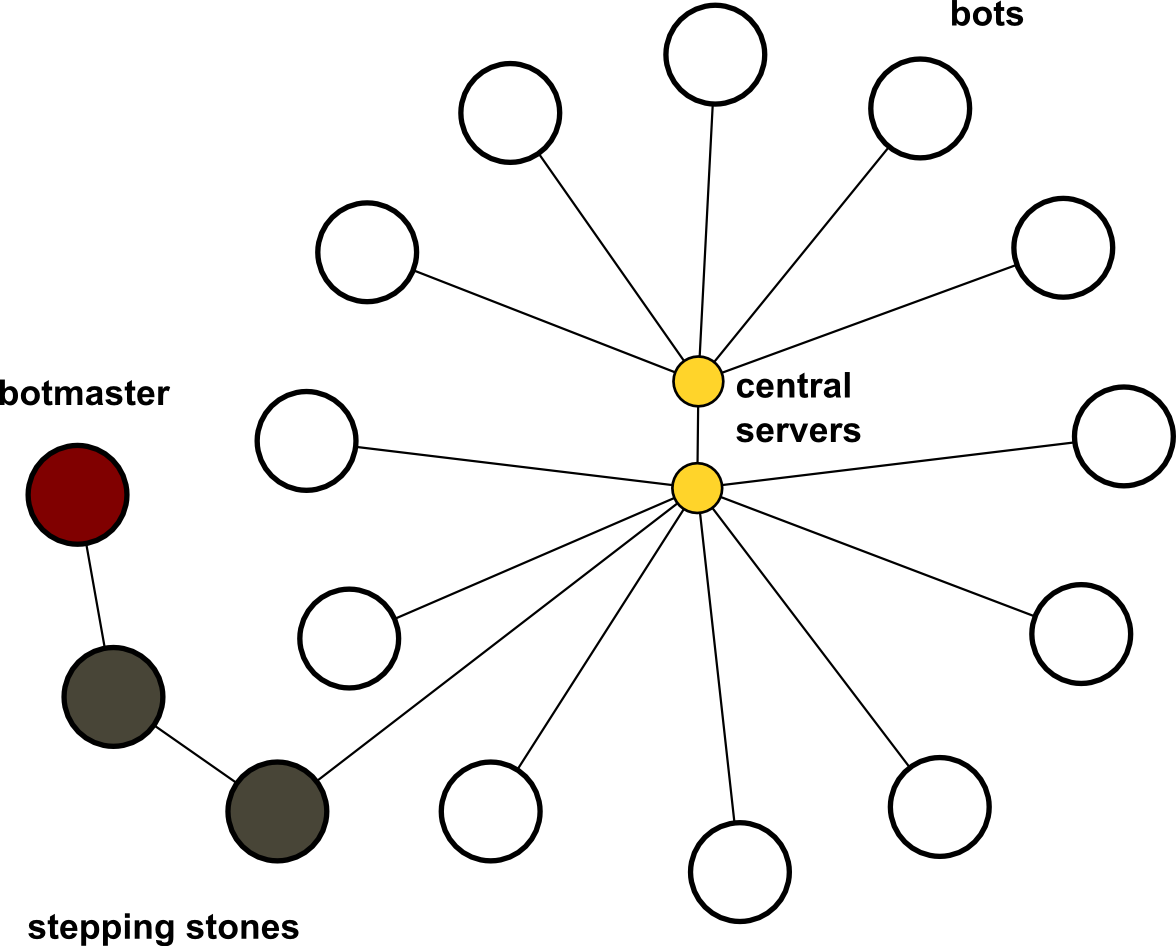
\includegraphics[width=0.8\textwidth]{figures/central-network.png}
  }
  \caption{Graph depicting connections in a centralized network. Note
    how all bots only have a connection to the central point. (Source:
    \cite{dittrich2007command})}
  \label{central-network}
\end{figure}
Historically the oldest form of botnets, centralized architectures are
built up in such a way that there is one central spot which broadcasts
messages between the connected bots and the botmaster. It functions
like a repeater. It's common to have more than one central
server\cite{td1sc}, but even with several servers, the architecture
still stays centralized. For if you shutdown this central point, the
network is inoperable. This resembles the biggest weakness of
centralized architectures: As soon as you are able to cut the server
off the net, the network lies arest. On the other hand, latency
becomes minimal, as the routing distance for one package needed to
reach each knode in the network is minimal (only one transition is
needed). Bandwidth, however, is generally limited by the server's
resources, making it hard to receive or transmit big chunks of
data. Furthermore, it holds that all the routes have the same length,
at least from the point of view of the botnet architecture graph.

Due to their nature, centralized architectures are usually implemented
with an IRC C\&C or similar\cite{cooke2005zombie}. The central server
is normally not owned by the botmaster. This would make detecting his
identity easy. In many countries, launching an ``evil-minded botnet''
is a serious crime. Instead, hacked or public IRC servers are used as
the central C\&C node. A connection from the attacker's computer to
the central server is often abufascated by many in-between relays,
tunnels and encryption. A sentence because of launching a botnet is
thus relatively seldom. Yet, in 2007 John Schiefer was sentenced to
four years in prison. He built a botnet with up to 250,000 zombies,
collecting passwords and bank credentials from the bots.  In figure
\ref{central-network} this is shown as the ``steeping stones'' which
shall hide an attacker's idenity.

\subsubsection{Decentralized Architecture}
\label{decent}
Dezentralized architectures do not rely on the special role of one
central server. Instead, they are built upon the principal of
equality, namely that the ``peer nodes (both client and server) are
all equal''\cite{steggink2007detection}. The topology of the network
is far more complex than in centralized architectures, forming a mesh
as shown in figure \ref{p2p-network}. It is thus more difficult for a
bot to join the botnet. Extensive bootstrapping is required, as the
bot has to figure out an already-participating peer to connect to in the
beginning. Once inside the net, information about other peers is
exchanged between knodes.Once inside the net, information about other peers is
exchanged between knodes. There are two approaches for bootstrapping\cite{wang2009systematic}:
\begin{itemize}
\item A list of peers likely to be online is hardcoded into the client. This list can later be updated
\item A shared web cache on the internet stores information about
  peers. The address of is hardcoded.
\end{itemize}

As can be seen, Bootstrapping is a critical and vulnerable point in
any P2P botnet. Considerable efforts by botmaster have been made to
circumvent the need to bootstrap\cite{td1sc}. This is further
discussed in \ref{counter-measure}.

Once inside the net, information about other peers is
exchanged between knodes.

Distributing commands and data in such a network is complicated, as it
has to be assured that the message reaches all clients. As a general
rule of thumb, the better inter-connected the knodes are, the higher
the probability for a message to reach all recipients.

This has the advantage of having the accumulated resources and
bandwidth of all the peers in the network available. However, latency
might be bad, as routing through the network is not trivial
(cf. figure \ref{p2p-network}). P2P networks are generally considerd
to be harder to disable (cf. section \ref{counter-measure} on page
\pageref{counter-measure}).

It is to be discussed whether P2P networks with a centralized server
architecture for certain services like file-indexing --- we refer to
them as ``Napster-like'' botnets --- fall into this
category. Principally, the connection graph differs a lot from
centralized networks, but they share the same weaknesses, as could be
seen when Napster was shut down in
2001\cite{napsterWiki}.\footnote{This was performed as an act of
  cofirming with the decision made in the intellectual property case
  of US A&M Records, Inc. v. Napster, Inc., 239 F.3d 1004 (2001) and
  not an explicit attack against the Napster network, but the fact
  that the Napster network could so easily stop the network by just
  disconnecting its central server shows the inherent weakness of
  centralized architectures.}  Dittrich et
al. \cite{dittrich2007command} would consider Napster-like botnets a
hybrid architecture, whereas Steggink et al.
\cite{steggink2007detection} classify it as
decentralized. 

\begin{figure}[htbp]
  \centering
  \fbox{
    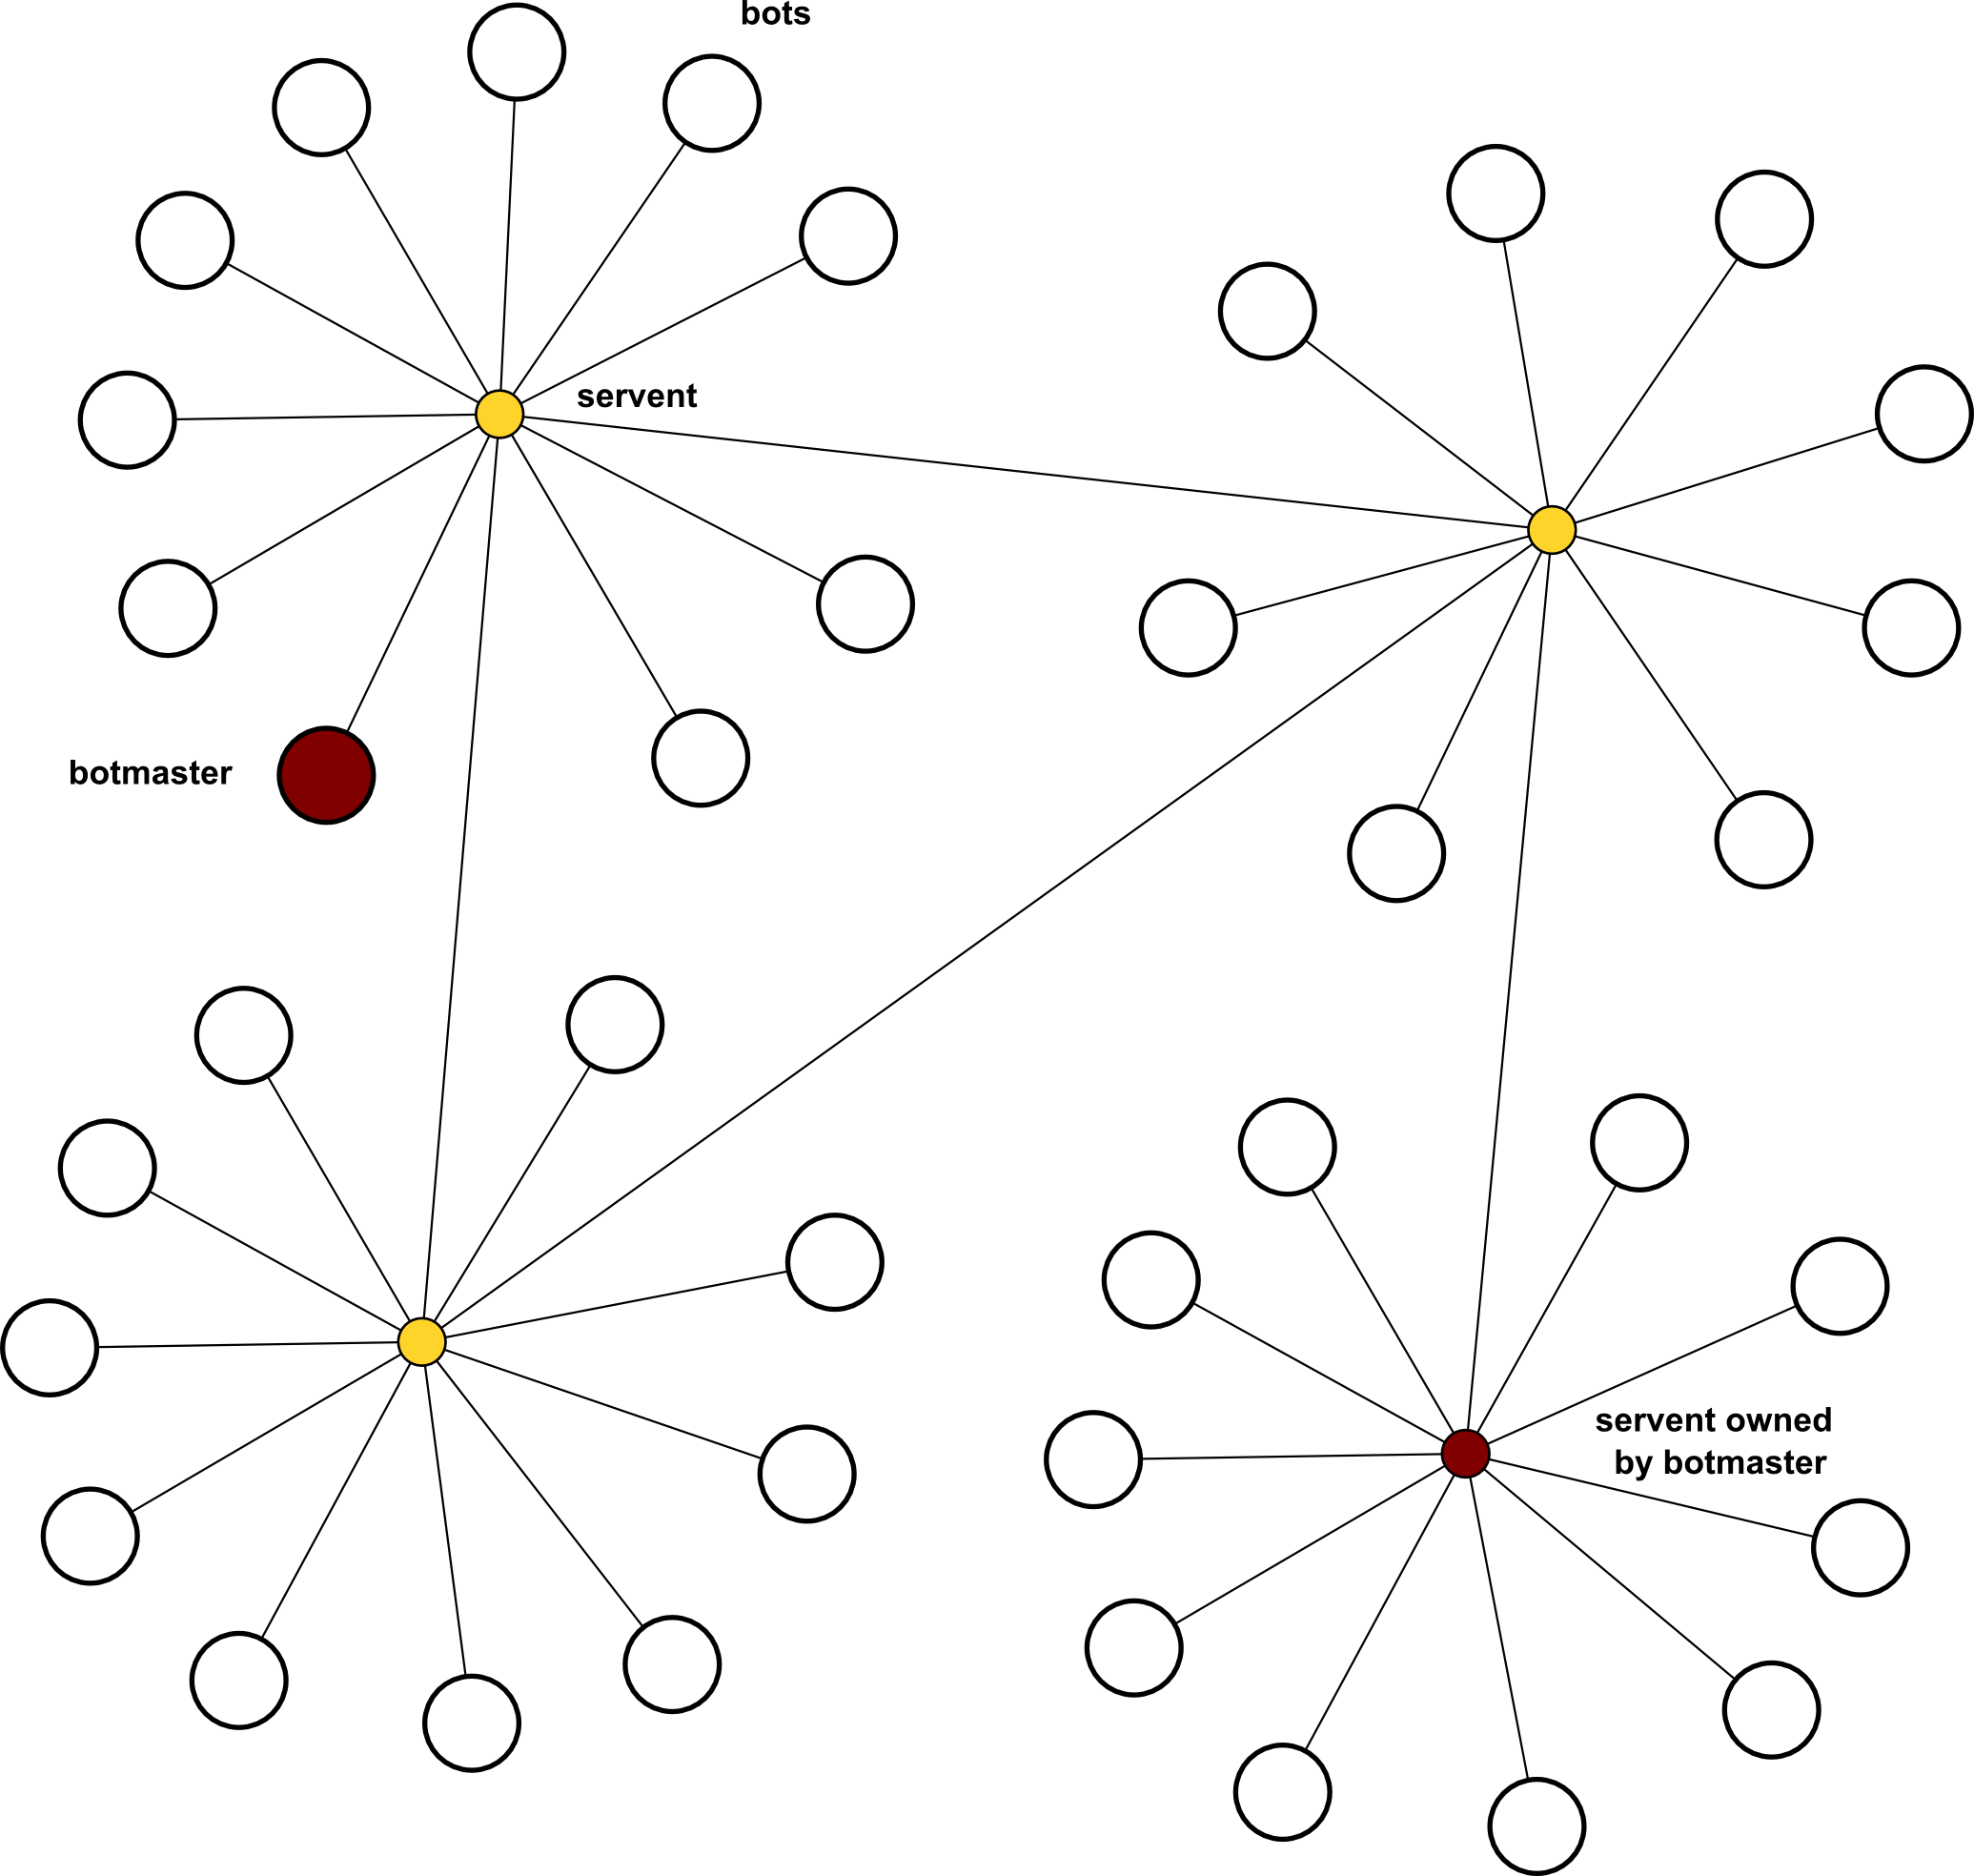
\includegraphics[width=0.7\textwidth]{figures/p2p-network.png}
  }
  \caption{P2P network (Source: \cite{dittrich2007command})}
  \label{p2p-network}
\end{figure}


\subsubsection{Hybrid Architecture}
\begin{figure}[htbp]
  \centering
  \fbox{
    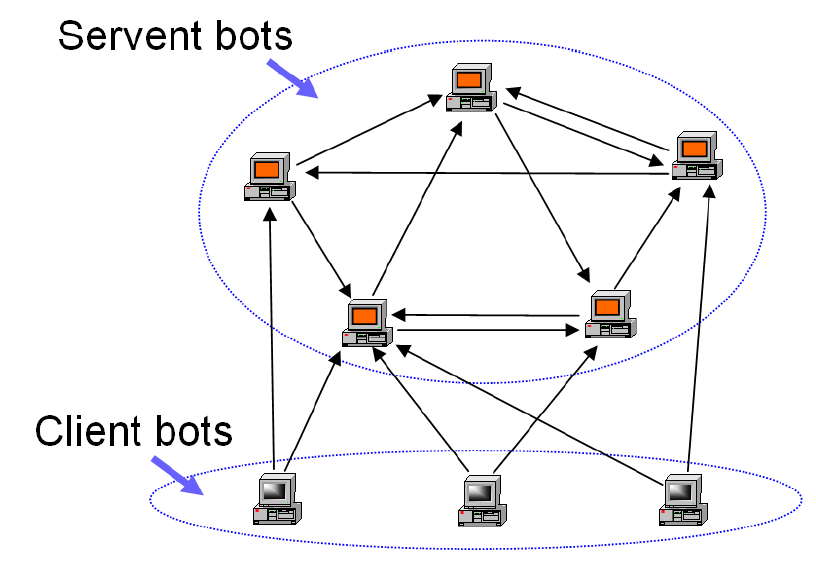
\includegraphics[width=0.7\textwidth]{figures/hybrid-network.png}
  }
  \caption{Hybrid network (Source: \cite{td1sc})}
  \label{hybrid-network}
\end{figure}
hele: \cite{td1sc}

doesnt need bootstrapping
fixed size peer list no reveal to others 
only static ip bots as peers -> no many deadlicks in peer list called servents (cf. figure)
separation between servents classically all bots (clients/servers) and clients: bots behind firewalls, private ips and dynamic ip
data encryption
Push/pull mechanism
peer list updating on update command by botmaster

super botnet vogt et all. not likely to become successful in a real world scenario as indicated by simulations in advanced ... degree of servent knodes vs. degree of initial servent bots


The advanced hybrid P2P botnet [10] and the super botnet [11] are two
newly designed P2P botnets, whose C\&C commu- nication are not
dependent on existing P2P protocols. Both of them implements push and
pull C\&C mechanisms. In a hybrid P2P botnet, when a bot receives a
command, it forwards the command to all the peers in the list (push),
and those who cannot accept connection from others periodically
contacts other bots in the list and try to retrieve new commands
(pull).  A super botnet is composed of a number of small centralized
botnets. Commands are pushed from one small botnet to (a) Centralized
Botnet (b) Index-based P2P Botnet Fig. 1: Similarity of logical C\&C
structures between traditional centralized botnets and index-based P2P
botnets another, and within a small centralized botnet, bots pull the
command from their C\&C servers. Furthermore, the hybrid P2P botnet is
able to effectively avoid bootstrap procedure, which is required by
most of the existing P2P protocols, by 1) passing a peer list from one
bot to a host that is infected by this bot, and 2) exchanging peer
lists when two bots communicate.  The drawback of designing a new
protocol for P2P botnet communication is that the new protocol has
never been tested before. When a botnet using this protocol is
deployed, the network may not be as stable and robust as expected due
to complex network conditions and defenses.

\cite{wang2009systematic}

\subsection{Lifetime of P2P botnets}
Wang et al.\cite{wang2009systematic} differentiate three stages of P2P botnets:
\begin{itemize}
\item recruiting bot members
\item forming the botnet
\item standing by for instruction
This is the actual ``operational'' phase of the botnet. Bots are awaiting instructions from their master. Instructions can either be actual commands or performing updates. In this phase, the chosen C\&C structure is essential.
\end{itemize}
It should be noted that these phases are not strictly exclusive,
e.g. during the third phase building of the botnet may well
continue. In fact, this is a typical property of any P2P network. It
is only until a critical mass of bots has proceeded past phase one and
two, that the botnet can be called operational.

\section{C\&C in P2P botnets}
Central server, hybrid, completely decentralized

Dezentralized: Peacom p.7 in 10.1.1.112.3561.pdf
see p. 3 in 10.1.1.153.8296

authentication of commands

push/pull distribution of c\&c

\section{Comparison: Conventional bots vs. P2P bots}

\section{Detection of and Counter measure against evil P2P botnets}
\label{counter-measure}
what to defend against
- detection
- in p2p: false commands from not botmaster
- shutdown of single hosts
- shutdown of large parts of botnet
- shutdown of whole botnet

Bootstrapping is a vulnerable point in any P2P botnet. When a hardcoded peer list is used (cf. for details), it is sufficient to take down all the peers in the bootstrapping table for the network to eventually shutdown: New bots simply can't find an initial peer to connect to. Botmasters have reacted to this by providing a Gnutella-like web-cache or updateable bootstrapping tables.

%------------------------------------------------------------------------------
\bibliographystyle{alpha}
\bibliography{literature}



\end{document}
